\section{Ergebnisse der Anordnungsvariation}\label{anhang:Anordnung}
In diesem Abschnitt werden die Ergebnisse der Variation der Anordnung dargestellt, die im Verlauf der Arbeit nicht weiter ausarbeitet wurden, da der Einfluss im späteren Einsatz nicht relevant erscheint.
\begin{figure}[htb]
    \centering
    \subfloat[1 Kurzschluss, Breite $\SI{30}{\milli\meter}$ ]{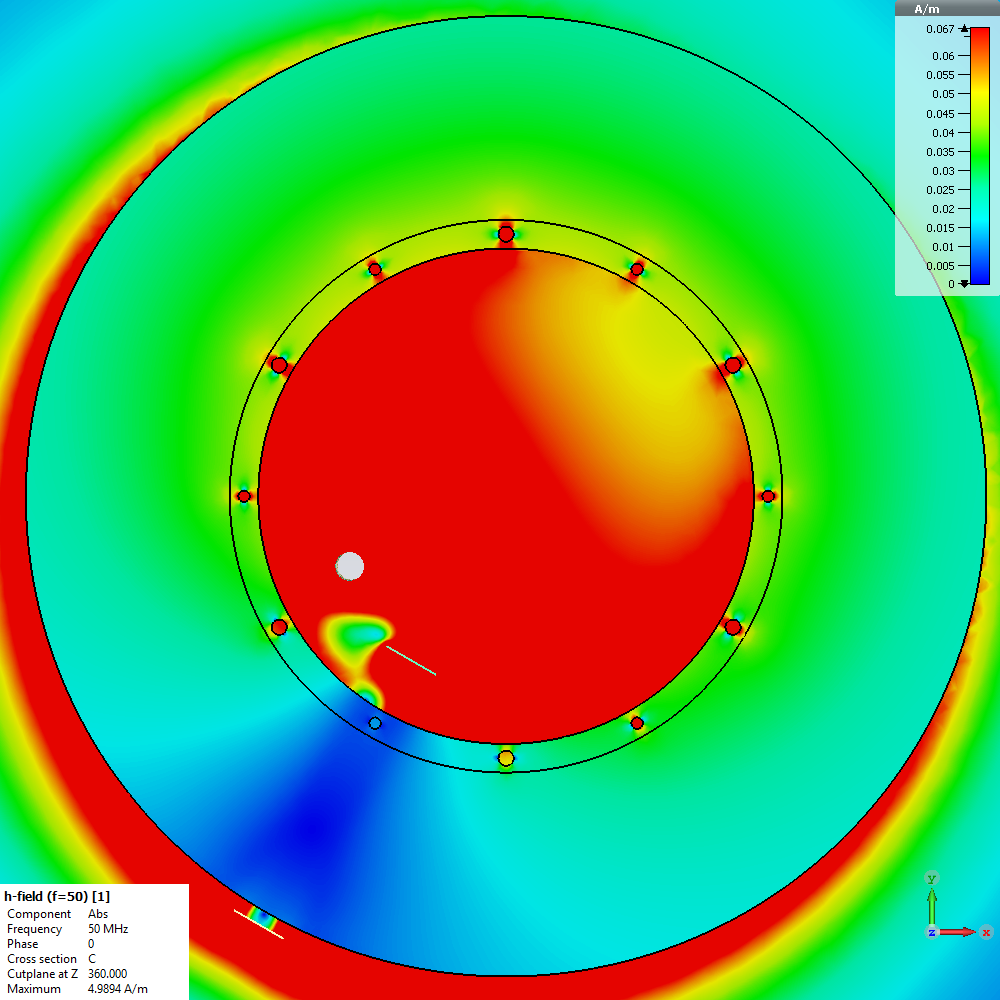
\includegraphics[width=0.33\textwidth]{Feldbilder/1KS}}
    \subfloat[2 Kurzschl\"usse, Breite $\SI{30}{\milli\meter}$]{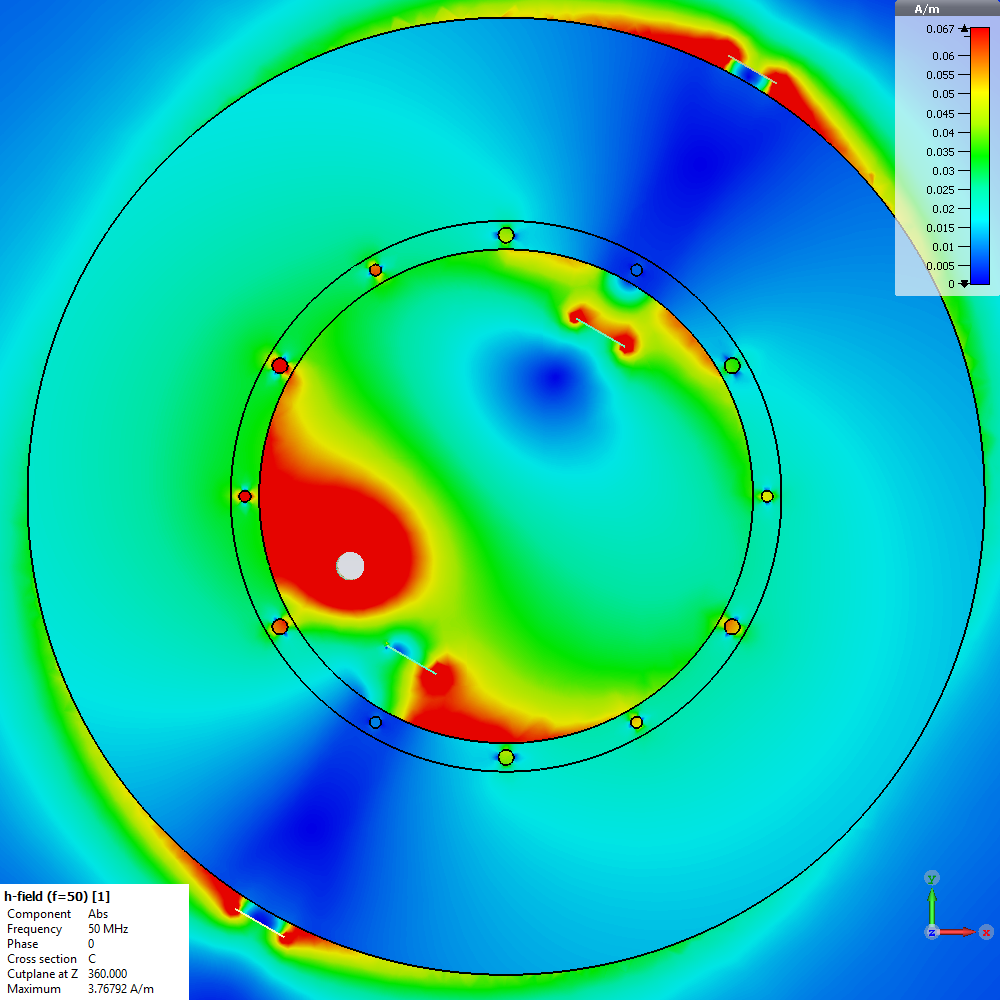
\includegraphics[width=0.33\textwidth]{Feldbilder/2KS}}
    
    \subfloat[1 Kurzschluss, Breite $\SI{50}{\milli\meter}$]{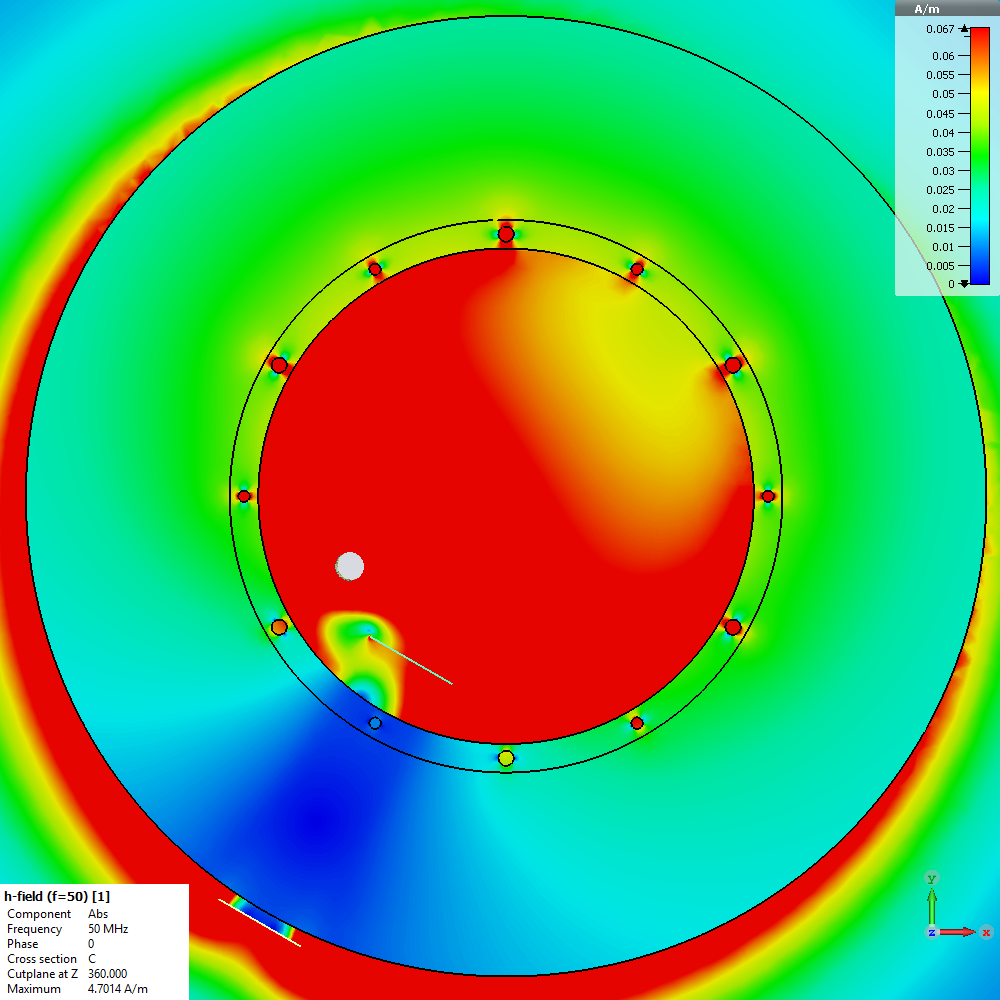
\includegraphics[width=0.33\textwidth]{Feldbilder/1KSb50}}
    \caption{Gegen\"uberstellung der Feldbilder für die Variation der Anordnung von Kurzschlüssen um den Ringkern, Länge der Kurzschlüsse $\SI{160}{\milli\meter}$}
    \label{fig:fieldAnordnung}
\end{figure}
